\documentclass{article}
\usepackage[left=2cm,right=2cm,top=2cm,bottom=2cm]{geometry}
\usepackage[utf8]{inputenc}
\usepackage[german]{babel}
\usepackage{amsmath}
\usepackage{dsfont}
\usepackage[export]{adjustbox}
\usepackage{amsthm}
\usepackage{color}
\usepackage{amsfonts}
\usepackage{amssymb}
\usepackage{wasysym}
\usepackage{makeidx}
\usepackage{graphicx}
\usepackage[colorlinks=true,urlcolor=blue,linkcolor=blue]{hyperref}
\usepackage{ziffer}
\usepackage{minted}
\usepackage{xcolor}
\usepackage{framed}
\usepackage{mdframed}
\usepackage{subfiles}
\usemintedstyle{emacs}

\definecolor{purp}{HTML}{9A72AC}
\definecolor{re}{HTML}{FC6255}
\definecolor{gre}{HTML}{83C167}
\definecolor{blu}{HTML}{58C4DD}
\definecolor{shadecolor}{rgb}{0.85,0.85,0.85}
\definecolor{bg}{rgb}{0.95,0.95,0.95}
\setlength{\parindent}{0em} 

\BeforeBeginEnvironment{minted}{\begin{mdframed}[linewidth =2 ,backgroundcolor=bg , linecolor=black, linewidth=0.5]}
\AfterEndEnvironment{minted}{\end{mdframed}}

\newtheorem{defi}{Definition}
\BeforeBeginEnvironment{defi}{\begin{mdframed}[linewidth =2 ,backgroundcolor=bg , linecolor=black, linewidth=0.5]}
\AfterEndEnvironment{defi}{\end{mdframed}}

\newcommand{\bsp}{\textbf{Beispiel}:}
%\newcommand{\task}{\textbf{Aufgabe}:}

\newcommand{\bol}[1]{\textbf{#1}}
\newcommand{\q}[1]{\glqq #1\grqq}
\newcommand{\DODO}[1]{\textbf{\textcolor{red}{DODO:}} #1 \\ \begin{center}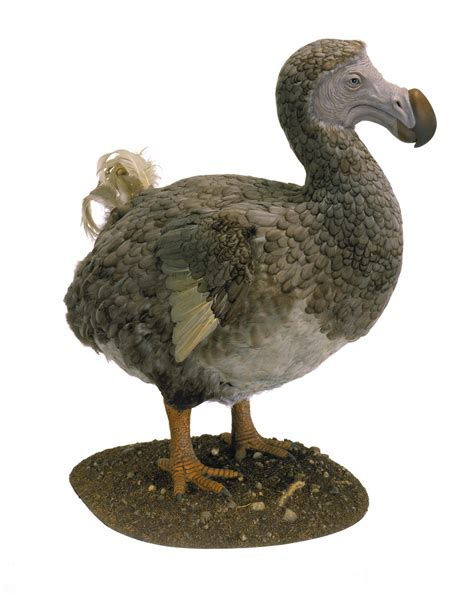
\includegraphics[scale=0.2]{../../media/dodo.jpg} \end{center}}

\newenvironment{task}[1]{
    \begin{shaded*}
    \textbf{Aufgabe #1}:
}{
    \end{shaded*}
}

\author{Lars Wechsler}
\title{Wiederholung wichtiger Grundbegriffe}

\date{\today}


\begin{document}
\maketitle

\section{Grundlegende Begriffe}

Die drei wohl grundlegensten Begriffe der objektorientierten Programmierung sind \q{Klasse}, \q{Objekt} und \q{Methode}.
\begin{task}{1}
Grenzen Sie die drei Begriffe mit Hilfe von Beispielen voneinander ab. 
\end{task}



\subsection{Klasse}
Die Klasse ist das zentrale Element der objektorientierten Programmierung, sie ist gewissermaßen ein \textbf{Bauplan} oder eine \textbf{Blaupause} für Objekte. Sie beschreibt alle Eigenschaften, die ein Objet dieser Klasse haben muss, gibt aber keine konkreten Werte vor. Eigenschaften werden in der Informatik \textbf{Attribute} genannt. Jedes Attribut hat einen bestimmten \textbf{Datentyp}, z.B.:
\begin{itemize}
    \item int
    \item double
    \item String
    \item boolean
\end{itemize}
Klassen werden häufig mit Hilfe von \textbf{Klassenkarten} visualisiert. Eine Klassenkarte besteht aus drei Segmenten, dem Klassennamen, den Attributen mit Datentypen und den Methoden (siehe unten), z.B.:
\begin{center}
    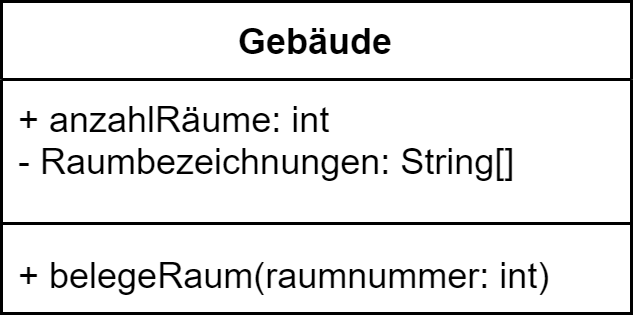
\includegraphics[scale=0.2]{../media/class.png}
\end{center}
In der Klassenkarte werden häufig neben den Datentypen auch noch die Sichtbarkeiten angegeben. Dabei steht $+$ für public, $-$ für private und $\#$ für protected. \\
Die konkrete Implementierung von Methoden findet keine Repräsentation in der Klassenkarte. Die Benennung der Methode sollte (wie auch die Benennungen der Attribute!) dafür sorgen, dass einem Programmierer, der diese Klasse implementieren soll, sofort klar ist, was die Methode tun soll. Deswegen gilt bei Benennungen die Faustregel:
\begin{center}
    So lange wie nötig, so kurz wie möglich. 
\end{center}
In Java gibt es die Konvention, dass Attribute (bzw. alle Variablen) und Methoden mit einem Kleinbuchstaben beginnen. Werden mehrere Worte aneinandergereiht, dann ohne Leerzeichen mit Großbuchstaben als Anfangsbuchstaben, wie bei \textit{anzahlRäume} im obigen Beispiel, im Fachbegriff heißt dies \bol{lower camel Case}. \\
Wird für jede Klasse eine Klassenkarte angegeben und deren Beziehungen untereinander dargestellt, so spricht man von einem Klassendiagramm (siehe auch Anhang Listenskript!) 
\newpage
\bol{Großes Beispiel} \\
\begin{center}
    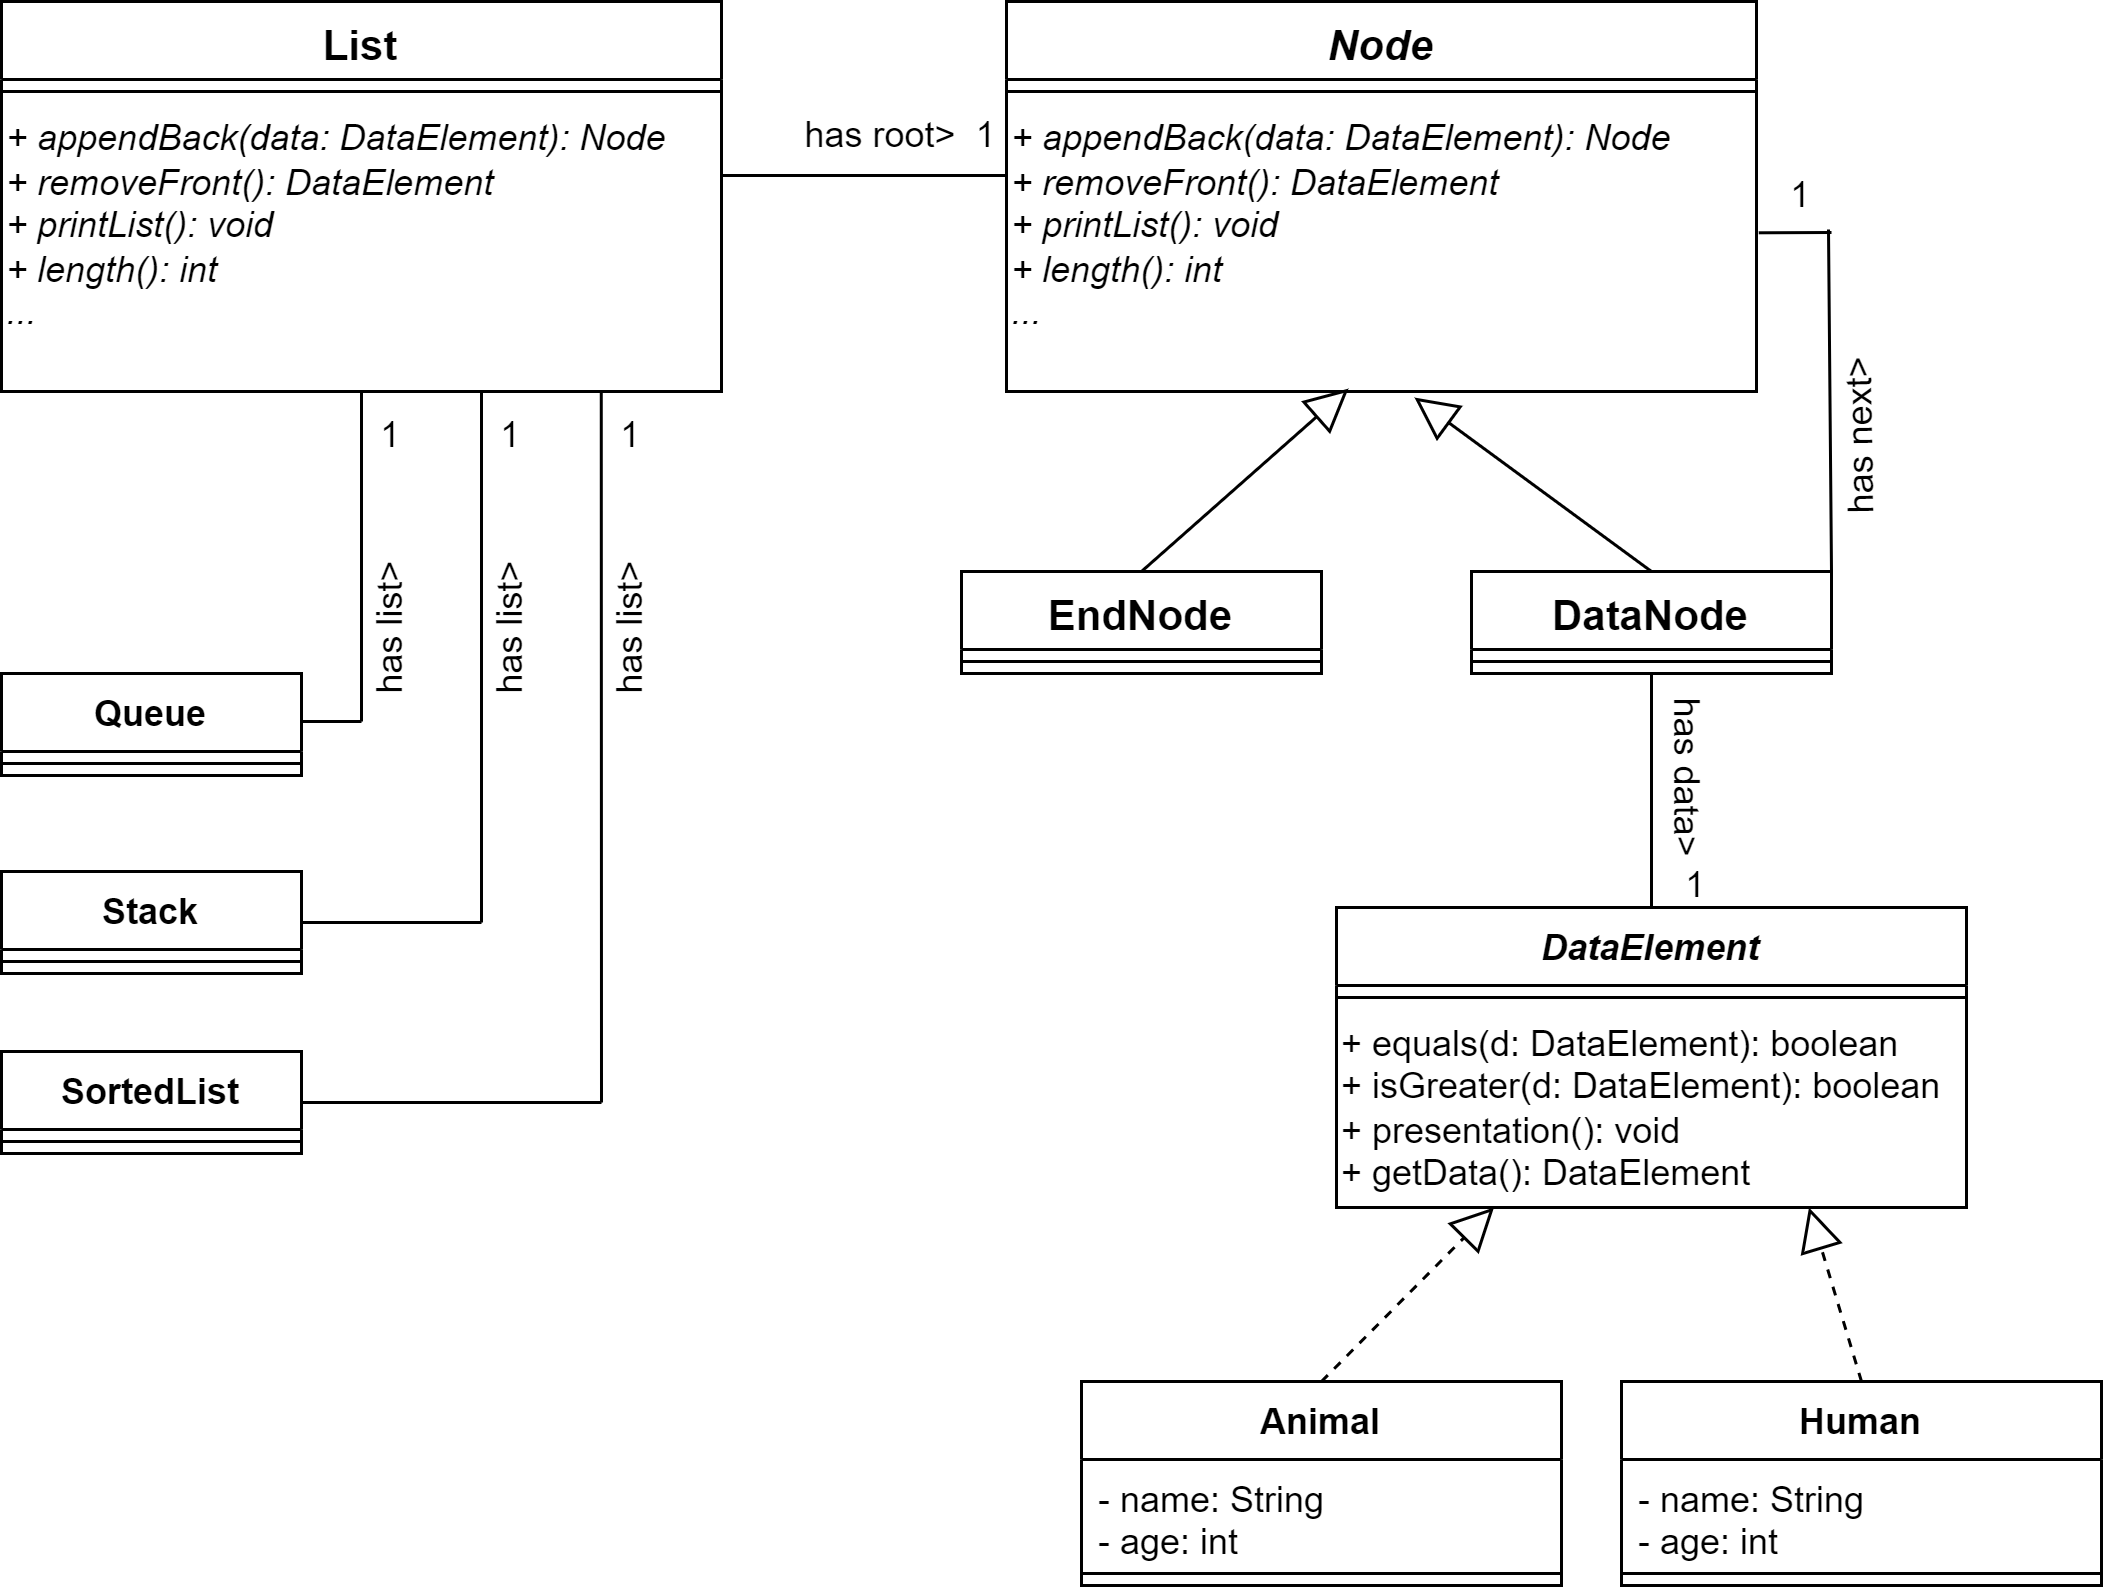
\includegraphics[scale=0.2]{../media/adapter_lists.png}
\end{center}

\subsection{Objekte}
Ein Objekt ist eine \textbf{Instanz} einer Klasse, d.h. eine konkrete Ausprägung des Bauplans der zugehörigen Klasse. (Es können z.B. auch mehrere Häuser nach demselben Bauplan gebaut werden, sich aber in einzelnen Eigenschaften, wie der Außenfarbe unterscheiden!). \\

In \textbf{Objektkarten} werden nicht mehr die Datentypen, sondern die konkreten Werte angegeben, außerdem werden keine Methoden mehr notiert. Um Objektkarten von Klassenkarten unterscheiden zu können, werden Objektkarten in der Schule mit abgerundeten Ecken dargestellt. Ein bestimmtes Gebäude der obigen Klasse könnte also so aussehen:
\begin{center}
    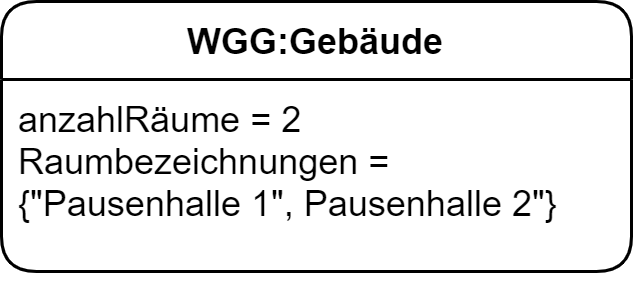
\includegraphics[scale=0.2]{../media/object.png}
\end{center}

\subsection{Methoden}
Methoden sind das Mittel zur Interaktion zwischen Objekten, Berechnungen oder salopp gesagt: ohne Methoden passiert nichts. Sie werden durch ihre \bol{Signatur} beschrieben:
\begin{minted}{Java}
    public String toLowercase(String input);
      (1)    (2)        (3)              (4)
\end{minted}
\begin{enumerate}
    \item Die \bol{Sichtbarkeit} verhält sich analog zur Sichtbarkeit von Attributen (auch bei Methoden kann private sinnvoll sein, wenn es sich z.B. um eine Hilfsmethode handelt, die nur innerhalb eines Objekts der Klasse verwendet wird). 
    \item Der \bol{Rückgabewert} gibt an, ob die Methode nach Beendigung etwas an den Methodenaufrufer zurückgibt. In diesem Fall wird ein String zurückgegeben, der in einer Variable gespeichert oder direkt weiter verwendet werden kann. (Erinnerung: kein Rückgabewert entspricht \q{void})
    \item Der \bol{Name} der Methode. Es gilt wie bei Attributen die Konvention, dass der lowerCamelCase verwendet wird und der Name möglichst aussagekräftig sein sollte (siehe oben).
    \item Für die \bol{Eingabeparameter} muss sowohl der Datentyp, als auch ein Variablenname für die lokale Verwendung innerhalb der Methode definiert werden. Die Übergabeparameter \q{verschwinden} nach Beendigung der Methode wieder aus dem Speicher, gibt es keinen Rückgabewert können sie also nicht \q{weiterverwendet} werden.
\end{enumerate}
\textit{Hinweis:} Streng genommen gehören in Java für den Compiler nur die Einträge 3 und 4 zur Signatur. Daraus folgt, dass die Kombination aus Name und Eingabeparameter (und hier auch nur deren Datentypen!) für eine Klasse immer eindeutig sein muss, andernfalls entsteht ein Fehler. (Das gilt natürlich nicht Klassenübergreifend, jede Klasse kann z.B. eine setName(String name) Methode haben, deren Implementierung sich unterscheiden. Erbt eine Klasse von einer anderen ist es sogar üblich, Methoden aus der Oberklasse mit derselben Signatur zu überschreiben, um neues Verhalten zu bekommen. Man spricht hier von Polymorphie) \\

\begin{task}{2}
Welche der folgenden Methoden können zusätzlich zur ersten in der Liste in einer Klasse existieren? \\
\end{task}

\begin{minted}{Java}
    public void magic(int a, int b) {
        //magic
    }

    public void magic(int c, int d) {
        //more magic
    }

    public int magic(int a, int b) {
        //integer magic?
    }

    public int magic(double a) {
        //double magic
    }

    public int magicTwo(int a, int b) {
        //double the magic
    }
\end{minted}
Wird eine zweite Methode mit gleichem Namen, aber unterschiedlichen Eingabeparametern definiert wird auch von \bol{Überladung} gesprochen. 
\newpage

\section{Referenzen und Kapselung}

Die Erzeugung von Objekten erscheint in Java recht umständlich und redundant, jeder Baustein erfüllt aber eine Funktion. Der Java Compiler verlangt vergleichsweise viele Informationen, da Java \bol{stark typisiert} ist, d.h. bereits beim compilen müssen z.B. Datentypen bekannt und klar festgelegt sein. \\
\textit{\bol{Hinweis:}} Python beispielsweise verlangt die starke Typisierung nicht. Das hat den Vorteil, dass die Syntax von Python weniger \q{überladen} aussieht, dafür fallen Fehler oft erst zur Laufzeit auf. \\
Wir nehmen an, es ist eine Klasse \textit{Circle} mit dem Attribut \textit{radius} mit einem entsprechenden Konstruktor implementiert, sowie einer weiteren Methode.
\begin{minted}{Java}
    public class Circle {
        private double radius;

        public Circle(double radius) {
            this.radius = radius;
        }

        public void enlarge(double toAdd) {
            radius += toAdd;
        }

    }
\end{minted}
Ein neuer Kreis wird in einer anderen Klasse (z.B. in einer Methode der Klasse Window) wie folgt \bol{instanziiert}, d.h. erzeugt: 
\begin{minted}{Java}
    public class Window {
        //... 
        public void greatMethod() {
            //... 
            Circle circle = new Circle(5.7);
            //(1)   (2)     (3)   (4)
        }
    }
\end{minted}
Die dreifache Verwendung des Wortes \q{Circle} in dieser Verwendung scheint exzessiv, jede hat aber eine Bedeutung: 
\begin{enumerate}
    \item Die starke Typisierung verlangt von uns, den Datentyp der folgenden Variable bzw. Referenz anzugeben. Der erste \q{Circle} verrät dem Compiler also, dass wir ein Objekt der Klasse Kreis haben wollen. 
    \item Die Benennung der Variable als \q{circle} ist natürlich nicht zwingend nötig, gerade bei einzelner Verwendung eines Objekts dieser Klasse aber durchaus üblich. Eine Variable ist letztendlich nichts anderes als eine Refernz auf einen bestimmten Ort im Speicher, an dem die gewünschten Informationen liegen. Die Speicherung von Informationen wird häufig mit dem \q{Kisten-Analogon} beschrieben. In einer Kiste werden Informationen (z.B. eine Zahl gepeichert). Diee Variable ist dann unsere Referenz (also das \q{Label} der Kiste) zu dieser Information. \\
    Im Unterschied zu primitiven Datentypen zeigt diese Referenz aber nicht auf z.B. eine Zahl direkt, sondern auf den Speicherort des Objekts, das wiederum aus vielen Teilinformationen bestehen kann, beispielsweise den Ausprägungen der Attribute. 
    \item new ist Javas Schlüsselwort, das für die Erzeugung neuer Objekte reserviert ist. 
    \item Der letzte \q{Circle} initiiert den Methodenaufruf des Konstruktors der Klasse Circle mit dem Parameter $5.7$. 
\end{enumerate}
\newpage
Wir benötigen die Referenz auf das Kreisobjekt, um öffentliche Methoden überhaupt aufrufen zu können. 
\begin{minted}{Java}
    public void greatMethod() {
        //... 
        Circle circle = new Circle(5.7);
        circle.enlarge(3);
    }
\end{minted}
Ohne die Referenz auf den Speicherorts des Kreises geht die Information verloren. Der Kreis hat keinen \q{eigenen Namen}, mit dem wir ihn im Speicher wiederfinden können, wenn wir die Referenz \textit{circle} zu ihm verlieren. \\ 
Ist die tolleMethode() also beendet, so verschwindet die Referenz \textit{circle} aus unserem Zugriffsbereich, da es sich um eine lokale Variable handelt. Objekte, zu denen keine Referenz mehr besteht werden in Java vom sogenannten \bol{garbage collector} \q{zerstört}. \\ 
Das \q{Denken in Referenzen} ist insbesondere auch bei Feldern wichtig. \\
\begin{minted}{Java}
    public class Window{
        /* 
        * Die Referenz circles verweist hier auf einen Ort im Speicher an dem 
        * weitere Referenzen zu den einzelnen Kreisen gespeichert sind. 
        */
        private Circle[] circles; 

        public Window(int amount) {
            circles = new circles[amount];
            for(int i = 0; i < circles.length; i++) {
                circles[i] = new Circle(5);
            }
        }

        /*
        * Mit Hilfe der im Feld gespeicherten Referenzen können wir 
        * alle Kreise vergrößern. 
        */
        public void enlargeCircles(double toAdd) {
            for(int i = 0; i < circles.length; i++) {
                circles[i].enlarge(toAdd);
            }
        }   
    }
\end{minted}
Eine ausführlichere Wiederholung der Felder findet sich auch im nächsten Skript. \\
Zurück zu einem einzelnen Kreis: Um das Attribut \textit{radius}  zu ändern, brauchen wir zwingend eine öffentliche Methode, da das Attribut als \textit{private} deklariert wurde. Das bedeutet, dass ein Zugriff von außerhalb des Objekts unmöglich ist. Dieses in der objektorientierten Programmierung übliche Konzept wird auch \bol{Kapselung} genannt. Für den Zugriff werden stattdessen getter- und setter-Methoden benutzt, z.B.: 
\begin{minted}{Java}
    public class Circle {
        private double radius;

        public Circle(double radius) {
            this.radius = radius;
        }

    public double getRadius(){
        return radius;
    }



    public void setRadius(double newRadius) {
        if(newRadius > 0) {
            radius = newRadius;
        }
    }
    }
\end{minted}
In diesem Beispiel verhindert die setRadius-Methode, dass ein negativer Radius gesetzt werden kann, da dieser im Kontext nicht sinnvoll wäre. 
\section{Welche Grundlagen müssen beherrscht werden?}
Hier noch einmal kompakt, welches Wissen als Voraussetzung gesehen wird:
\begin{itemize}
    \item Grundlegendes theoretisches Wissen zu Klassen, Objekten und Methoden.
    \item Grundlagen zur Vererbung.
    \item Sichere Verwendung von Referenzen, Konstruktoren und Methodenaufrufen. 
    \item Implementierung einfacher Klassen, insbesondere mit gettern und settern.
    \item Implementierung einfacher Methoden im Kontext, siehe Aufgabe.
\end{itemize}

\begin{task}{3}
    \\
a) Implementieren sie eine Klasse Würfel (Dice), die die Methode int würfeln() (int rollDice()) besitzt. Zusätzlich soll sich ein Objekt die letzte gewürfelte Zahl \q{merken} können. \\
b) Schreiben Sie eine Klasse Spiel (Game), deren Konstruktor eine vorgegebene Menge an Würfeln in einem Feld speichert. \\
c) Ergänzen Sie eine Methode int augensumme() (int eyeSum()), die jeden Würfel einmal würfeln lässt und anschließend die Augensumme zurückgibt. \\
d) Schreiben Sie eine Methode void letzterWurf() (void lastRoll()), die für jeden Würfel auf der Konsole den Wert des letzten Wurfs ausgibt. Ergänzen Sie dazu notwendige Methoden in der Klasse Würfel. 
\end{task}
Auf der nächsten Seite findet sich eine (!) mögliche Lösung der Aufgaben.
\newpage

\begin{minted}{Java}
    public class Dice {
        private int lastRoll; 

        public int rollDice() {
            int random = (int) Math.round(Math.random()*5 + 1);
            lastRoll = random;
            return random;
        }

        public int getLastRoll() {
            return lastRoll;
        }
    }

    public class Game {
        private Dice[] dice;

        public Game(int diceAmount) {
            dice = new Dice[diceAmount];
            for(int i = 0; i < diceAmount; i++) {
                dice[i] = new Dice();
            }
        }

        public int eyeSum() {
            int sum = 0;
            for(int i = 0; i < dice.length; i++) {
                sum += dice[i].rollDice();
            }
            return sum;
        }

        public void lastRoll() {
            for(int i = 0; i < dice.length; i++) {
                System.out.println("Dice " + i + " has rolled " + dice[i].getLastRoll());
            }
        }
    }
\end{minted}
\end{document}